% Model 1 couples daily root-zone water with annual cover.
\subsection{Coupled Vegetation--Water--Sand Dynamics}\label{sec:model1}
\subsubsection[Daily Water Balance and Annual Vegetation Growth]{Model construction}
\paragraph{Two states on two timescales.} Annual cover $V_t$ sets daily transpiration demand $D_j$. We divide the monthly forcing and assigned irrigation evenly among the days of each month and update plant-available root-zone water $M_j$ in mm at each step. At year end, the fraction of demand met drives the cover update, and the remaining water carries into the next year (Figure~\ref{fig:m1-clocks}).

\begin{figure}[!htb]
  \centering
  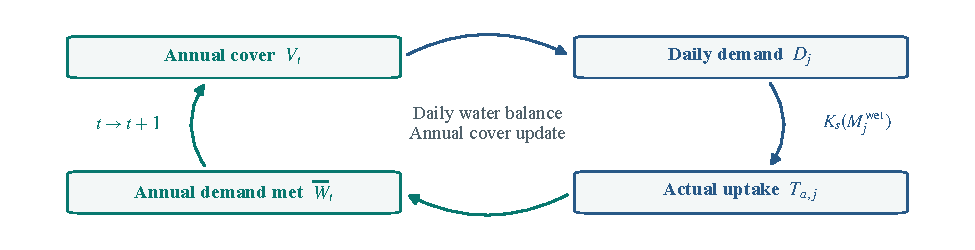
\includegraphics[width=\linewidth]{../Figures/Paper2026_Mechanisms/m1_water_feedback.pdf}
  \caption{Daily water uptake and annual cover feedback.}
  \label{fig:m1-clocks}
\end{figure}

\paragraph{Cover equation: growth and decay.}
\begin{equation}\label{eq:m1-veg}
V_{t+1}=V_t+\underbrace{rV_t\Big(1-\frac{V_t}{K}\Big)\overline W_t}_{\text{growth, limited by water}}
-\underbrace{dV_t}_{\text{natural decay}}
\end{equation}
\emph{Growth} is logistic, stops at the local ceiling $K$, and is scaled by the water-satisfaction ratio $\overline W_t\in[0,1]$ (Eq.~\eqref{eq:m1-wbar}). \emph{Decay} removes a fixed share $d$ of cover each year. There is no separate wind term; wind enters through the water demand below. Since $V=0$ stays at $0$, every scenario starts from a planted cover.

\paragraph{Root-zone water balance.} Add the effective fractions of rain and irrigation to the starting store $M_j$ and drain water above capacity $C$ (Figure~\ref{fig:m1-bucket}). The resulting available store is $M_j^{\mathrm{wet}}$:
\begin{equation}\label{eq:m1-bucket}
M_j^{\mathrm{wet}}=\min\!\big(C,M_j+\alpha_PP_j+\eta_wI_j\big),\qquad
T_{a,j}=\min\!\big(M_j^{\mathrm{wet}},K_sD_j\big),\qquad
M_{j+1}=M_j^{\mathrm{wet}}-T_{a,j}.
\end{equation}
The daily demand and the stress coefficient are
\begin{equation}\label{eq:m1-demand}
D_j=c\,\min\!\Big(1,\frac{2V_t}{V_{\mathrm{full}}}\Big)\,f(T_j)\,\mathrm{ET}_{0,j},\qquad
K_s=\min\Big\{1,\ \frac{M_j^{\mathrm{wet}}}{(1-p)C}\Big\}.
\end{equation}
The transpiration coefficient $c$ scales reference evapotranspiration $\mathrm{ET}_0$ to stand demand. Demand rises with cover up to $V_{\mathrm{full}}/2$. The seasonal factor $f(T)$ is zero at or below $5\,^\circ\mathrm{C}$ and reaches one at $25\,^\circ\mathrm{C}$. The FAO-56 coefficient $K_s$ limits uptake below the baseline available-water threshold of $37.5$\,mm~\cite{REF11}. Figure~\ref{fig:m1-stress} shows both multipliers, with 2015--2022 monthly mean temperatures from Yutian and Minfeng marked on $f(T)$.

\begin{figure}[!htbp]
  \centering
  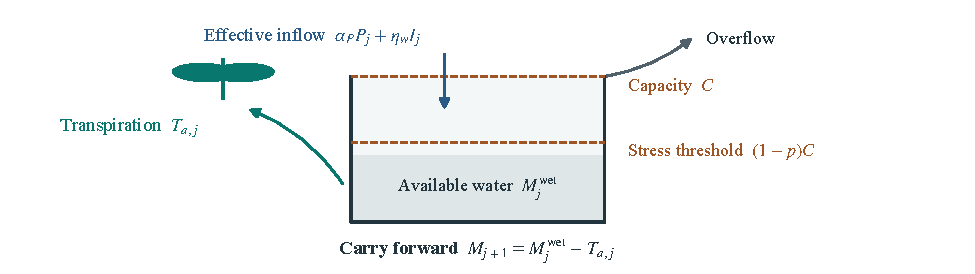
\includegraphics[width=\linewidth]{../Figures/Paper2026_Mechanisms/m1_root_zone.pdf}
  \caption{One daily step of the root-zone water balance.}
  \label{fig:m1-bucket}
\end{figure}

\begin{figure}[!htbp]
  \centering
  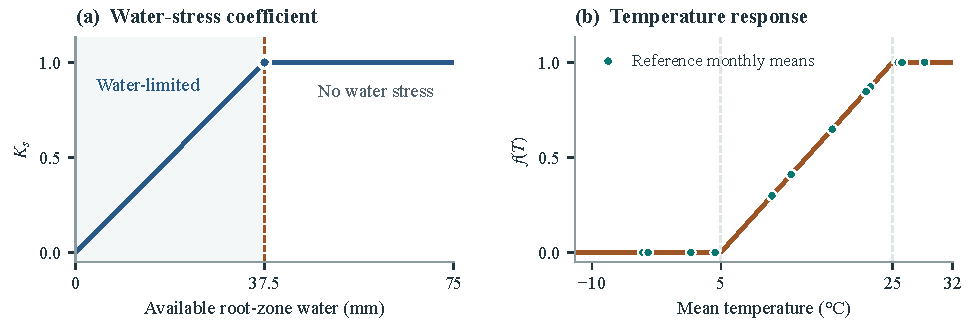
\includegraphics[width=\linewidth]{../Figures/Paper2026_Polished/fig05_stress_switches.pdf}
  \caption{Water-stress and temperature response functions.}
  \label{fig:m1-stress}
\end{figure}

\paragraph{The link between the two clocks.} The daily bucket and the yearly cover update are coupled through one number, the water-satisfaction ratio
\begin{equation}\label{eq:m1-wbar}
\overline W_t=\frac{\sum_{j\in t}T_{a,j}}{\sum_{j\in t}D_j},
\end{equation}
the share of plant water demand actually met in year $t$. No water stress ($\overline W_t=1$, as in oases) yields full growth rate $r$; intermediate values scale growth proportionally ($\overline W_t=0.4$ reduces growth to $0.4\,r$); and $\overline W_t=0$ halts growth, leaving only decay.

\paragraph{Wind: water demand and disaster damage.} We distinguish two pathways. In Model~1, day-to-day wind affects growth through evaporative demand. The reference evapotranspiration $\mathrm{ET}_0$ in Eq.~\eqref{eq:m1-demand} follows FAO-56 Penman--Monteith \cite{REF11},
\begin{equation}\label{eq:m1-pm}
\mathrm{ET}_0=\frac{0.408\,\Delta\,(R_n-G)+\gamma\,\dfrac{900}{T+273}\,u_2\,(e_s-e_a)}{\Delta+\gamma\,(1+0.34\,u_2)},
\end{equation}
where $u_2$ is the wind speed at 2\,m, $R_n-G$ the available energy, $e_s-e_a$ the dryness of the air, and $\Delta$, $\gamma$ thermodynamic coefficients. At baseline, the aerodynamic term accounts for 61\% of annual reference $\mathrm{ET}_0$. Wind speed enters both the numerator and the denominator, so this share differs from the response to changing wind speed. A windier climate therefore raises the demand $D_j$, lowers $\overline W_t$ and slows growth.

In Model~1, the index $S_t=E_t(1-V_t/K)$ tracks relative sand exposure: higher cover leaves less surface exposed. We use $S_t$ only as a diagnostic because the annual observations cannot isolate direct wind damage to vegetation. Model~3 treats direct cover loss from severe storms separately.

The growing-season weighting reduces annual reference demand from 1,686 to 1,191\,mm/yr (Figure~\ref{fig:m1-sens}a). At long-run quotas of 300 and 600\,mm/yr, year-end storage remains below the stress threshold.

\subsubsection[Least-Squares Calibration and Long-Run Simulation]{Solution approach}
We fit growth and decay from data, step the coupled system through a year, and repeat the year to reach a long-run state or a scenario path.

\paragraph{Step 1: calibration by least squares.} At the seven oasis stations water is ample ($\overline W\approx1$), so we set $\overline W=1$ there; growth and decay can then be estimated from cover alone. Fixing $K$ from each station's own record and writing $x=V/K$, Eq.~\eqref{eq:m1-veg} becomes
\begin{equation}\label{eq:m1-reg}
\underbrace{x_{s,t+1}-x_{s,t}}_{y_{s,t}:\ \text{observed change}}=r\,\underbrace{x_{s,t}(1-x_{s,t})}_{z_{1,s,t}:\ \text{growth signal}}-d\,\underbrace{x_{s,t}}_{z_{2,s,t}:\ \text{decay signal}}+\varepsilon_{s,t},
\end{equation}
where $s$ indexes stations and $\varepsilon_{s,t}$ is the one-step error. The model is linear in the unknowns $(r,d)$, so we estimate them by ordinary least squares over the set $\mathcal T$ of training pairs (target year $\le2022$, all seven stations pooled):
\begin{equation}\label{eq:m1-ls}
(\hat r,\hat d)=\arg\min_{r,d}\ \sum_{(s,t)\in\mathcal T}\big(y_{s,t}-(r\,z_{1,s,t}-d\,z_{2,s,t})\big)^2 .
\end{equation}
We solve Eq.~\eqref{eq:m1-ls} with design matrix $\bm Z=[\,\bm z_1,-\bm z_2\,]$. To estimate uncertainty, we resample whole stations with replacement, keeping each station's time series intact, and refit $(r,d)$ for each bootstrap sample.

\paragraph{Steps 2--3: one model year, then repeat.} Algorithm~\ref{alg:m1} shows the core loop. Repeating it under a typical climate year until $V$ and $M$ stop changing gives the long-run state for a given irrigation level. Because $\overline W$ depends on $V$, this fixed point is found numerically; we start from both a low and a high cover and accept the result only when both starts agree.

\begin{algorithm}[H]
\caption{One model year: the water store drives cover}\label{alg:m1}
\begin{algorithmic}[1]
\Require cover $V_t$, store $M$, irrigation $I_t$, monthly rain, ET$_0$ and temperature
\Ensure $V_{t+1}$, year-end store $M$, $\overline W_t$
\State Set daily demand $D_j$ from $V_t$ and the season \Comment{cover held fixed}
\For{each day $j$ of the year}
  \State $M\gets M+\alpha_PP_j+\eta_wI_j$;\quad spill anything above $C$ \Comment{inflow subtract overflow}
  \State $T_{a,j}\gets\min\big(M,K_s(M)D_j\big)$;\quad $M\gets M-T_{a,j}$ \Comment{water index is stressed when $M$ is low}
\EndFor
\State $\overline W_t\gets\sum_jT_{a,j}/\sum_jD_j$ \Comment{Eq.~\eqref{eq:m1-wbar}}
\State $V_{t+1}\gets$ Eq.~\eqref{eq:m1-veg};\quad carry $M$ into next year
\end{algorithmic}
\end{algorithm}

\begin{table}[H]
\centering\small
\caption{Parameter values for Model 1.}
\label{tab:m1-par}
\renewcommand{\arraystretch}{1.1}
\begin{tabularx}{\linewidth}{@{}l X r c l@{}}
\toprule
Symbol & Meaning & Value & Range tested & Unit \\
\midrule
\multicolumn{5}{@{}l}{\textit{Fitted by least squares (Eq.~\eqref{eq:m1-ls})}}\\
$r$ & intrinsic growth rate & 0.547 & 0.335--1.168$^{\dagger}$ & yr$^{-1}$ \\
$d$ & natural decay rate & 0.107 & 0.077--0.202$^{\dagger}$ & yr$^{-1}$ \\
\midrule
\multicolumn{5}{@{}l}{\textit{Set from data by a fixed rule}}\\
$K$ & cover ceiling ($1.15\times$ 95th percentile of training cover) & 38.08 & -- & \% \\
$V_{\mathrm{full}}$ & oasis end-member used to scale demand & 66.59 & 64.85--69.40 & \% \\
\midrule
\multicolumn{5}{@{}l}{\textit{Assumed}}\\
$C$ & root-zone storage capacity & 75 & 30--150 & mm \\
$p$ & stress-free share of storage (FAO-56 \cite{REF11}) & 0.5 & 0.3--0.7 & -- \\
$c$ & transpiration coefficient & 1.0 & 0.7--1.2 & -- \\
$\eta_w$ & share of irrigation reaching the roots (FAO-56 \cite{REF11}) & 0.75 & 0.65--0.85 & -- \\
$\alpha_P$ & share of rain reaching the roots (FAO-56 \cite{REF11}) & 0.25 & 0--1 & -- \\
$u_T$ & wind threshold in the index $E_t$ & 5 & -- & m/s \\
$V_0$ & initial cover of a new stand & 2 & -- & \% \\
$M_0$ & initial store of a new stand & 37.5 & -- & mm \\
\bottomrule
\end{tabularx}
\end{table}

\subsubsection[Vegetation Response to Irrigation and Wind]{Results}

\paragraph{Model reliability.} Across the 21 held-out site-years, one-step RMSE in $V/K$ is 0.0635 for Model~1 and 0.0536 for persistence. The model improves on persistence at the two reference sites, Yutian and Minfeng, but has larger errors at the other five (Figure~\ref{fig:m1-obs}a). A free run from 2022 illustrates the limitation at Ruoqiang: predicted cover is 33.0\% in 2025 against 38.4\% observed (panel d). We therefore use Model~1 to compare irrigation strategies.

\begin{figure}[!htbp]
  \centering
  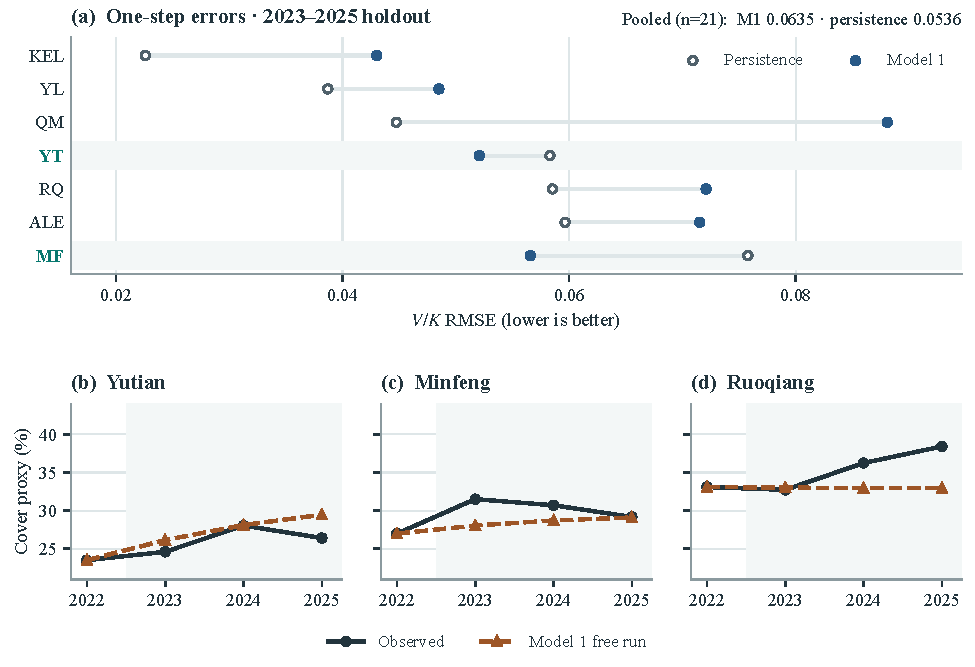
\includegraphics[width=\linewidth]{../Figures/Paper2026_Polished/fig06_holdout.pdf}
  \caption{Holdout errors and cover trajectories.}
  \label{fig:m1-obs}
\end{figure}

\paragraph{Evolution of the state variables.} From a planted cover of 2\%, cover and soil water pass through three phases (Figure~\ref{fig:m1-curve}b,d):
\begin{enumerate}\setlength{\itemsep}{1pt}\setlength{\parsep}{0pt}
  \item \textbf{Establishment: growth, not water, limits cover.} Young plants use little water. All plotted quotas of 300\,mm/yr or more meet demand ($\overline W=1$) through 2030 and reach 9.9\% cover at year-end. Extra irrigation does not increase cover in this phase.
  \item \textbf{Transition: cover drains the store.} Demand rises with cover until it exceeds supply. The store then drops from capacity within about two years and settles slowly (to about 13.5\,mm at 300\,mm/yr), and $\overline W$ falls below one. This is the feedback at work: more cover means less water per plant, which slows growth.
  \item \textbf{Plateau (after 15--25 years): both settle.} By 2050, cover and year-end storage are near their plateaus: 17.9\% and 13.5\,mm at 300\,mm/yr, and 24.1\% and 19.3\,mm at 600\,mm/yr.
\end{enumerate}
Trajectories repeat 2015--2022 weather. In the stop scenario, irrigation is 600\,mm/yr through 2035. In the first year after irrigation stops, year-end storage falls from 22.8 to 0.81\,mm and $\overline W$ falls to 0.045. Cover falls from 21.5\% to 12.7\% after five years and to 5.1\% after fifteen years.

\paragraph{Controlling factors: water supply.} Water supply is the main control. Without irrigation, annual rainfall of 52\,mm against roughly 1,700\,mm of reference evaporative demand sustains only 1.8\% long-run cover in the model.

The first 100\,mm/yr adds 7.7 percentage points of long-run cover, while increasing the quota from 500 to 600\,mm/yr adds only 1.6 points. At 300\,mm/yr only 37\% of demand is met. Beyond about 1,500\,mm/yr, additional water overflows and the cover proxy levels off at 30.6\% (Figure~\ref{fig:m1-curve}a,c).

\begin{figure}[!htbp]
  \centering
  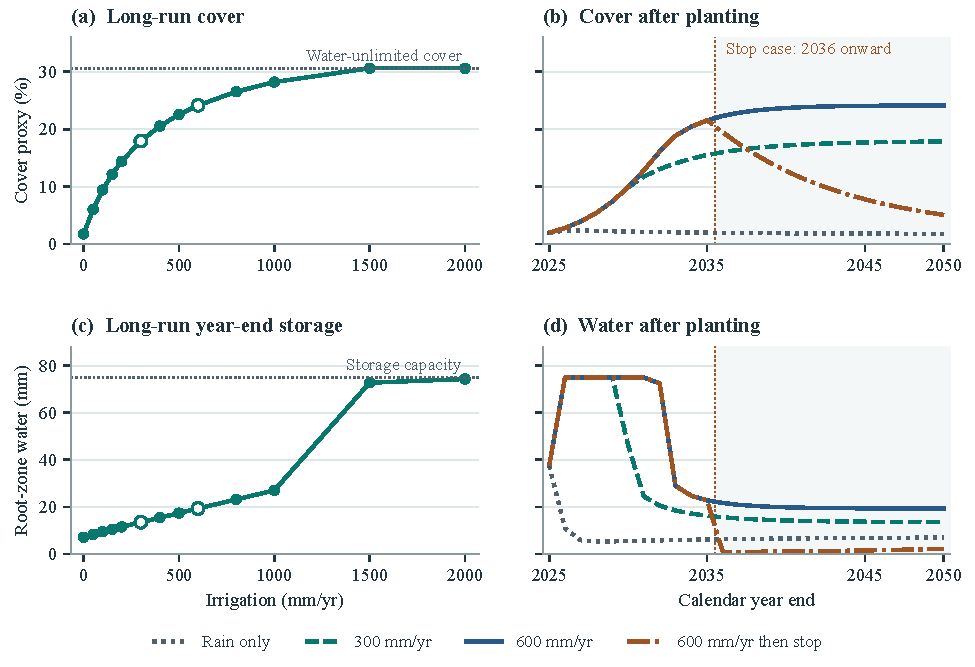
\includegraphics[width=\linewidth]{../Figures/Paper2026_Polished/fig07_irrigation_response.pdf}
  \caption{Cover and root-zone storage under alternative irrigation schedules.}
  \label{fig:m1-curve}
\end{figure}

\paragraph{Controlling factors: demand, delivery and wind.} With water supply fixed, we varied the other factors one at a time (Figure~\ref{fig:m1-sens}). They fall into three groups:
\begin{enumerate}\setlength{\topsep}{1pt}\setlength{\itemsep}{0pt}\setlength{\parsep}{0pt}
  \item \textbf{Factors that shift long-run cover by 1--3 points:} the transpiration coefficient $c$ ($-1.7$ to $+3.4$ points at 300\,mm/yr), irrigation efficiency ($\pm1.2$) and the effective rain fraction ($-0.5$ to $+1.4$). All three act through $\overline W$, the supply-to-demand ratio.
  \item \textbf{Factors that change soil water but not long-run cover:} storage capacity and the stress threshold. Without overflow, all inflow is eventually transpired, so $\overline W$ depends only on inflow and demand; these factors change only the storage level and its timing.
  \item \textbf{Wind, through evaporative demand.} Scaling wind speed in Eq.~\eqref{eq:m1-pm} by $+20\%$ raises season-adjusted reference demand by 7.7\% and lowers long-run cover at 300\,mm/yr from 17.9\% to 17.2\%; $-20\%$ raises it to 18.8\% (Figure~\ref{fig:m1-sens}b). Less cover leaves more sand exposed: $S$ moves from 0.53 to 0.55.
\end{enumerate}
\begin{figure}[!htbp]
  \centering
  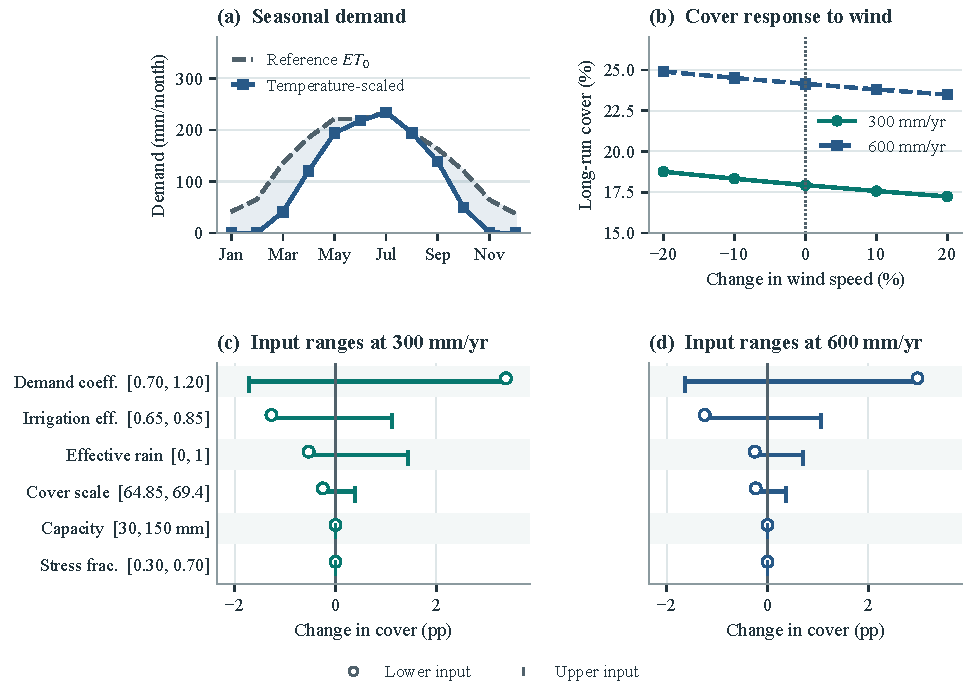
\includegraphics[width=\linewidth]{../Figures/Paper2026_Polished/fig08_drivers.pdf}
  \caption{Demand, wind response and drivers of long-run cover.}
  \label{fig:m1-sens}
\end{figure}

\paragraph{Summary.} Cover and soil water rise together, settle at a level set by the water supply, and decline once water stops. Water supply is the main control, with sharply diminishing returns. Wind acts through the water demand: 20\% more wind costs about 0.7 points of cover, and cover in turn decides how much sand stays exposed.

